% Электронный учебник будет представлять собой один файл в формате pdf.
% Для того, чтобы создать этот
% файл, нужно поработать с настоящим документом, который в дальнейшем будем называть
% <<рабочий файл>>. Прежде, чем приступать к работе, прочтите внимательно первые две части
% <<Руководства пользователю>>. По большому счету электронное издание <<Руководство
% пользователю>> показывает стиль и
% структуру создаваемого электронного учебника (стиль и структуру, конечно же, можно будет
% поменять по Вашему усмотрению). Основную часть экрана занимает так называемая рабочая
% область -- здесь будет представлена информация учебника, предназначенная для изучения
% студентами. Правая часть -- интерактивная панель, предназначенная для удобной навигации
% по документу.

% Теперь можно приступать к работе. Внимательно читайте все комментарии (они начинаются после
% символа %).
% Если Вы что-нибудь поменяли, то для того, чтобы увидеть результат,
% нужно скомпилировать рабочий файл в pdf-документ (см. <<Руководство пользователю>>).

%---------------------------------------------------------------------------------------------------------------

\documentclass[12pt, a4paper]{book}% Эту команду не стоит менять
\usepackage{xspace,colortbl}% Эту команду не стоит менять
\usepackage[utf8]{inputenc}% Эту команду не стоит менять
\usepackage[english,russian]{babel}% Эту команду не стоит менять
\usepackage{euscript,latexsym,amsfonts,amsthm,amsmath,amssymb}% Эту команду не стоит менять
\usepackage[pdftex,hypertex]{hyperref}% Эту команду не стоит менять
\usepackage{color}% Эту команду не стоит менять
\usepackage[screen,panelright,sectionbreak]{pdfscreen}% Эту команду не стоит менять
\graphicspath{{images/}{images/amblems/}{images/fon/}{images/panel/}{images/pic/}}% Эту
% команду не стоит менять. Она указывает путь к папкам, в которых хранятся графические файлы
 \margins{.25in}{.25in}{.25in}{.30in}% Эту команду не стоит менять
 \screensize{6.25in}{8in}% Эту команду не стоит менять
  \changeoverlay% Эту команду не стоит менять
\usepackage{longtable}% Эту команду не стоит менять

\usepackage{graphicx}%Вставка картинок правильная
\usepackage{float}%"Плавающие" картинки
\usepackage{wrapfig}%Обтекание фигур (таблиц, картинок и прочего)

\usepackage{regexpatch}
\usepackage{listings}
\definecolor{keyword}{RGB}{0,0,150}
\definecolor{identifier}{RGB}{0,0,0}
\definecolor{comment}{RGB}{128,128,128}
\definecolor{string}{RGB}{0,128,0}
\definecolor{numbers}{RGB}{128,128,128}
\lstdefinestyle{customjava}{
  belowcaptionskip=1\baselineskip,
  breaklines=true,
  frame=L,
  xleftmargin=\parindent,
  language=java,
  numbers=left,
  showstringspaces=false,
  basicstyle=\small\ttfamily,
  numberstyle=\color{numbers},
  keywordstyle=\bfseries\color{keyword},
  commentstyle=\itshape\color{comment},
  identifierstyle=\color{identifier},
  stringstyle=\color{string},
}
\lstset{escapechar=@,style=customjava}
\makeatletter
\xpatchcmd*\@Overlay@Hook{\put(\strip@pt\@tempdima,\strip@pt\@tempdima)}
{\put(\strip@pt\@tempdima,\strip@pt\dimexpr.5\paperheight)}{}{}
\makeatother

%--------------------------------------------------------------------------------------------

 \paneloverlay{but3.png}% Аргумент этой команды, записанный в фигурных скобках, можно
% изменить. <<{but3.png}>> -- это имя графического файла, который используется в качестве
% фона интерактивной панели. Здесь можно прописать имя любого рисунка в формате png или pdf,
% который Вы хотите использовать в качестве фона для интерактивной панели. Файл
% этого рисунка должен находиться в папке Images/Panel.

%---------------------------------------------------------------------------------------------------

\overlay{m1.png} % Аргумент этой команды, записанный в фигурных скобках, можно
% изменить. <<{m8.png}>> -- это имя графического файла, который используется в качестве
% фона основой рабочей области. Здесь можно прописать имя любого рисунка в формате
% png или pdf, который Вы хотите использовать в качестве фона для основной рабочей области.
% Файл этого рисунка должен находиться в папке Images/fon.

%---------------------------------------------------------------------------------------------

\def\panel{\begin{minipage}[t][\paperheight][t]{\panelwidth}% Эту команду не стоит менять
\centering\null\vspace*{12pt}% Эту команду не стоит менять
 \par\vspace{0.3cm}% Эту команду не стоит менять

%---------------------------------------------------------------------------------------------

\includegraphics[width=2.54cm]{favicon_ru_RU.png}\par\vspace{0.6cm}% Эта команда позволяет вставить
% любую картинку в качестве эмблемы в верхней части интерактивной панели. Аргумент команды
% в квадратных скобках <<[width=2.54cm]>> задает ширину эмблемы (в сантиметрах),
% а аргумент команды в фигурных скобках <<{univ.png}>> -- это имя графического файла,
% содержащего саму эмблему. Здесь можно прописать имя любого рисунка в формате
% png или pdf, который Вы хотите использовать в качестве эмблемы.
% Файл этого рисунка должен находиться в папке Images/amblems
\vspace{0mm}% Эта команда задает расстояние (в миллиметрах) до следующей после эмблемы строки
{\LARGE\itshape Кафедра}% Эту команду лучше не менять

{\large\itshape ИИ}% Впишите сюда название Вашей кафедры

\vspace{5mm}% Эта команда задает расстояние (в миллиметрах) до первой кнопки
% интерактивной панели
%---------------------------------------------------------------------------------------------------

 \Acrobatmenu{FirstPage}{\addButton{1.05in}{\FBlack\@Начало}}\par\vspace{3mm} % Эта команда создает
% кнопку <<Начало>> на интерактивной панели. Нажатие этой кнопки возвращает пользователя
% на первую (титульную) страницу электронного учебника. Аргумент команды <<{\FBlack\@Начало}>>
% можно поменять (например, написать вместо <<Начало>> <<Пачатак>> или <<Титульная страница>>).

%------------------------------------------------------------------------------------------------

\hyperref[oglo]{{\addButton{1.05in}{\@Содержание}}}\par\vspace{3mm} %Эта команда создает
% кнопку <<Содержание>> на интерактивной панели. Нажатие этой кнопки возвращает пользователя
% на первую страницу раздела <<Содержание>> электронного учебника.
% Аргумент команды <<{\@Содержание}>> можно поменять (например, написать
% вместо <<Содержание>> <<Змест>> или <<Оглавление>>).

%---------------------------------------------------------------------------------------------

\hyperref[mybutton]{\addButton{1.05in}{\@Ваша кнопка}}\par\vspace{3mm}%Эта команда создает
% кнопку <<Ваша кнопка>> на интерактивной панели. Нажатие этой кнопки вернет пользователя
% на ту страницу электронного учебника, на которую Вы захотите. Для этого нужно в определенное
% Вами место любого раздела электронного учебника поставить метку \label{mybutton} (подробнее
% о метках можно прочитать в <<Руководстве пользователю>>). Обратите внимание, что имя этой
% метки должно совпасть с аргументом команды, записанном
% в квадратных скобках (\hyperref[mybutton]).
% Аргумент команды <<{\@Ваша кнопка}>> нужно поменять (написать
% вместо <<Ваша кнопка>> любой текст, указывающий пользователю, какую информацию он
% получит, нажав на эту кнопку). Такого типа кнопки удобно создавать для быстрого
% доступа пользователя к некоторой информации электронного учебника (например, справочной
% информации, перечню формул, и т.д.). При желании таких кнопок можно создать несколько
% (сколько позволит высота Интерактивной панели). Для этого нужно соответствующее
% число раз скопировать и вставить сразу после этого комментария
% команду \hyperref[imyametki]{\addButton{1.05in}{\@Ваша кнопка}}\par\vfill
% Если же Вы не хотите создавать ни одной своей кнопки, удалите всю строку, содержащую
% описываемую здесь команду и весь текст данного комментария.

%--------------------------------------------------------------------------------------------

\Acrobatmenu{PrevPage}{\addButton{.51in}% Не меняйте эту команду. Она создает кнопку перехода
{\FBlack\scalebox{.8}[1.4]{\btl}}}\hspace{1pt}% на одну страницу назад
\Acrobatmenu{NextPage}{\addButton{.51in}% Не меняйте эту команду. Она создает кнопку перехода
{\LBlack\scalebox{.8}[1.4]{\rtl}}}\par\vspace{3mm}% на одну страницу вперед

%---------------------------------------------------------------------------------------------

\Acrobatmenu{FirstPage}{\addButton{.51in}% Не меняйте эту команду. Она создает кнопку быстрого
{\FBlack\scalebox{.8}[1.4]{\btl\btl}}}\hspace{1pt}% перехода на первую страницу
\Acrobatmenu{LastPage}{\addButton{.51in}% Не меняйте эту команду. Она создает кнопку быстрого
{\LBlack\scalebox{.8}[1.4]{\rtl\rtl}}}\par\vspace{3mm}% перехода на последнюю страницу

%---------------------------------------------------------------------------------------------

\Acrobatmenu{GoToPage}{\addButton{1.05in}% Не меняйте эту команду. Она создает кнопку,
{\@Страница~\thepage~\@из~\pageref*{pages_total}}}\par\vspace{3mm}% позволяющую совершать
% переход на любую страницу электронного учебника

%---------------------------------------------------------------------------------------------

\Acrobatmenu{GoBack}{\addButton{1.05in} {\@Назад}}\par\vspace{3mm}% Не меняйте эту команду. Она
% создает удобную кнопку возврата к той странице электронного учебника, с которой был совершен
% переход по любой гиперссылке текста учебника или по некоторой кнопке Интерактивной панели.
% Аргумент команды <<{\@Назад}>> можно поменять (например написать вместо <<Назад>>
% <<Обратно>> или <<Возврат>>).

%---------------------------------------------------------------------------------------------------

\Acrobatmenu{FullScreen}{\addButton{1.05in}{\@На весь экран}}\par\vspace{3mm}% Эту команду лучше
% не менять. Она создает кнопку, позволяющую <<развернуть>> электронный учебник на весь экран.
% Аргумент команды <<{\@На весь экран}>> можно поменять (например написать вместо
% <<На весь экран>> <<Развернуть>> или <<Увеличить>>)

%---------------------------------------------------------------------------------------------

\Acrobatmenu{Quit}{\addButton{1.05in}{\@Закрыть}}\par\vspace{3mm}% Эту команду лучше
% не менять. Она создает кнопку, нажатие которой закрывает электронный учебник. Аргумент
% команды <<{\@Закрыть}>> можно поменять (например написать вместо
% <<Закрыть>> <<Выход>> или <<Уйти>>)

%---------------------------------------------------------------------------------------------

\end{minipage}}% Эту команду не стоит менять

\definecolor{panelbackground}{gray}{.8}% Эту команду не стоит менять
  \definecolor{buttonbackground}{gray}{.9}% Эту команду не стоит менять
  \definecolor{buttonshadow}{gray}{.2}% Эту команду не стоит менять
  \definecolor{orange}{rgb}{1,.549,0}% Эту команду не стоит менять
  \definecolor{orange1}{rgb}{1,.5,0}% Эту команду не стоит менять
  \definecolor{section0}{rgb}{0,.5,.1}% Эту команду не стоит менять
  \definecolor{section1}{rgb}{0,.5,1}% Эту команду не стоит менять
  \definecolor{section2}{rgb}{0,.5,.5}% Эту команду не стоит менять
  \definecolor{section3}{rgb}{0,.5,.4}% Эту команду не стоит менять
  \definecolor{section4}{rgb}{.4,.5,.2}% Эту команду не стоит менять
  \definecolor{section5}{rgb}{.5,.5,.3}% Эту команду не стоит менять
\newcommand{\esup}{\mathop{\rm ess\:sup\;}_{t>0\;\,}}% Эту команду не стоит менять
\newcommand{\res}{\mathop{\rm res}}% Эту команду не стоит менять
\renewcommand{\Re}{{\rm Re}}% Эту команду не стоит менять
\renewcommand{\Im}{\operatorname{Im}}% Эту команду не стоит менять
\newcommand{\norm}[1]{\left\Vert#1\right\Vert}% Эту команду не стоит менять
\newcommand{\set}[1]{\left\{#1\right\}}% Эту команду не стоит менять
\newcommand{\h}{{\mathcal H}}% Эту команду не стоит менять
\newcommand{\nur}{\EuScript{L}_{\nu,r}}% Эту команду не стоит менять
\newcommand{\nutwo}{\EuScript{L}_{\nu,2}}% Эту команду не стоит менять
\newcommand{\eqdef}{\stackrel{\rm def}{=}}% Эту команду не стоит менять
\renewcommand{\thesection}{\arabic{chapter}.\arabic{section}\hspace{-4mm}}% Эти команды не стоит менять
\renewcommand{\thesubsection}{\arabic{chapter}.\arabic{section}.% Эту команду не стоит менять
\arabic{subsection}\hspace{-4mm}}% Эту команду не стоит менять
\renewcommand{\theequation}{\arabic{chapter}.\arabic{equation}}% Эту команду не стоит менять
\makeatletter% Эту команду не стоит менять
\newcommand*\l@struct{\@dottedtocline{1}{0em}{2.3em}}% Эту команду не стоит менять
\newcommand{\l@abcd}[2]{\rightskip=\@pnumwidth\leftskip=% Эту команду не стоит менять
\@tempdima\hspace{-2.7em}\noindent #1\hfill% Эту команду не стоит менять
\rlap{\makebox[\@pnumwidth][r]{\bf#2}}}% Эту команду не стоит менять
\renewcommand*\l@section{\@dottedtocline{1}{1.5em}{2.2em}}% Эту команду не стоит менять
\renewcommand*\l@subsection{\@dottedtocline{2}{3.8em}{3.0em}}% Эту команду не стоит менять
\renewcommand{\section}{\@startsection{section}{1}{1pt}% Эту команду не стоит менять
{4.0ex plus -0.2ex minus -0.2ex}{2.0ex plus 0.2ex}{\centering\bf}}% Эту команду не стоит менять
\renewcommand{\subsection}{\@startsection{subsection}{2}% Эту команду не стоит менять
{23pt}{3.5ex plus -0.2ex minus -0.2ex}{1ex plus 0.2ex}{\bf}}% Эту команду не стоит менять
\renewcommand{\chapter}{\vspace{8mm}\global\@topnum=0% Эту команду не стоит менять
\@afterindenttrue\secdef\@chapter\@schapter}% Эту команду не стоит менять
\renewcommand{\@makechapterhead}[1]{{\parindent=0pt\raggedright% Эту команду не стоит менять
\bf ЛЕКЦИЯ { }\centering\Large\thechapter\vspace{0.1mm}~\centering% здесь можно заменить
% слово <<ЛЕКЦИЯ>> на любое другое

\large\bf #1\par\nopagebreak\vspace{4mm}}}% Эту команду не стоит менять

\renewcommand{\tableofcontents}{\section*{\contentsname}\@starttoc{toc}}% Эту команду не
% стоит менять

%--------------------------------------------------------------------------------------------

% Следующие команды задают вид и структуру раздела <<Содержание>> (этот раздел
% генерируется автоматически).
\def\@chapter[#1]#2{\ifnum \c@secnumdepth >\m@ne% Эту команду не стоит менять
\if@mainmatter% Эту команду не стоит менять
\refstepcounter{chapter}% Эту команду не стоит менять
\typeout{\@chapapp\space\thechapter.}% Эту команду не стоит менять
\addcontentsline{toc}{chapter}% Эту команду не стоит менять
{{\rm Лекция \,\thechapter}\ \ #1}% Здесь можно заменить слово <<Лекция>> на любое другое
\else% Эту команду не стоит менять
\addcontentsline{toc}{chapter}{#1}% Эту команду не стоит менять
\fi% Эту команду не стоит менять
\else% Эту команду не стоит менять
\addcontentsline{toc}{chapter}{#1}% Эту команду не стоит менять
\fi% Эту команду не стоит менять
\chaptermark{#1}% Эту команду не стоит менять
\addtocontents{lof}{\protect\addvspace{10\p@}}% Эту команду не стоит менять
\addtocontents{lot}{\protect\addvspace{10\p@}}% Эту команду не стоит менять
\if@twocolumn% Эту команду не стоит менять
\@topnewpage[\@makechapterhead{#2}]% Эту команду не стоит менять
\else% Эту команду не стоит менять
\@makechapterhead{#2}% Эту команду не стоит менять
\@afterheading% Эту команду не стоит менять
\fi}% Эту команду не стоит менять

\makeatother% Эту команду не стоит менять

%--------------------------------------------------------------------------------------------

% Следующие команды определяют имена окружений типа <<Теорема>> (см. <<Руководство
% пользователю>>).
% Аргумент команды \newtheorem, записанный в фигурных скобках -- это имя окружения,
% которое будет использоваться при записи команды, создающей соответствующее окружение
% в тексте электронного учебника, а поэтому оно должно состоять из латинских символов;
% команда \color{red} задает цвет надписи имени окружения на русском языке
% (доступные цвета: red (красный), gray (серый), orange (оранжевый), blue (голубой),
% green (зеленый) и т.д).
% Можно создавать свои собственные окружения такого типа. Например, команда
% \newtheorem{mymicl}{\indent \color{red}Моя мысль}[chapter] создаст окружение
% типа <<Теорема>> с именем <<Моя мысль>>.
\newtheorem{theorem}{\indent \color{red}Теорема}[chapter]
\newtheorem{lemma}{\indent \color{red}Лемма}[chapter]
\newtheorem{corollary}{\indent \color{red}Следствие}[chapter]
\newtheorem{note}{\indent \color{red}Замечание}[chapter]
\newtheorem{opr}{\indent \color{red}Определение}[chapter]
\newtheorem{example}{\indent \color{red}Пример}[chapter]
\newtheorem{utv}{\indent \color{red}Утверждение}[chapter]
\newtheorem{gip}{\indent \color{red}Гипотеза}[chapter]

%--------------------------------------------------------------------------------------------

\pagestyle{empty}% Эту команду не стоит менять



% Теперь вся подготовительная работа проведена, стиль и структура электронного
% учебника заданы. Дальше можно начинать наполнение электронного учебника.

% -----------------------------------------------------------------------------------------

\begin{document}\large% Эту команду не стоит менять
% Приступим к созданию титульной страницы. Далее можно менять все, что написано
% на русском языке. Но не забывайте читать комментарии.
\begin{center}% Эту команду не стоит менять. Она <<центрирует>> текст, заключенный между
% командами \begin{center} и \end{center}, по ширине экрана.
  УЧРЕЖДЕНИЕ ОБРАЗОВАНИЯ\\
  <<Брестский государственный технический университет>>
\end{center}% Эта команда завершает <<центрирование>> текста
\vspace{20mm}% Эта команда увеличивает расстояние между строками (расстояние указано
% в фигурных скобках в миллиметрах).
\begin{center}% Эту команду не стоит менять. Она <<центрирует>> текст, заключенный между
% командами \begin{center} и \end{center}, по ширине экрана.
\textbf{% Эта команда задает полужирный шрифт текста, являющегося аргументом
% команды (т.е. текста, заключенного в фигурные скобки)
     {\LARGE \color{red} СИСТЕМНОЕ ПРОГРАММНОЕ ОБЕСПЕЧЕНИЕ}\\[10mm]% Переход на следующую строку
% задан командой \\, а в квадратных скобках указано расстояние
% до следующей строки текста (в миллиметрах).
    \\[10mm]% Переход на следующую строку задан командой \\,
% а в квадратных скобках указано расстояние до следующей строки текста (в миллиметрах).
    {\it\Large Электронный учебно-методический комплекс }\\% Переход на следующую строку
% задан командой \\
    {\it\Large для студентов факультета электронно-информационных систем}% Любую из строк такого вида можно
% при желании удалить или добавить новую с произвольным текстом.
}
\end{center}% Эта команда завершает <<центрирование>> текста
\vspace{30mm}% Эта команда увеличивает расстояние между строками (расстояние указано
% в фигурных скобках в миллиметрах).
\begin{center}% Эту команду не стоит менять. Она центрирует текст, заключенный между
% командами \begin{center} и \end{center}, по ширине экрана.
Брест\\% Переход на следующую строку задан командой \\
БрГТУ\\% Переход на следующую строку задан командой \\
  2023% Здесь указывается год создания электронного учебника
\end{center}% Эта команда завершает <<центрирование>> текста

% --------------------------------------------------------------------------------------------

\newpage% Эта команда задает переход на новую страницу (разрыв страницы).

% На этой странице будет размещена информация об авторах, рецензентах, экспертах и т.д.
% Прежде, чем приступать к работе с этой страницей,
% прочитайте часть 3 <<Руководства пользователю>>.

 \overlay{m1.png}% Эта команда задает новый фон рабочей области. Аргумент этой команды,
% записанный в фигурных скобках, можно  изменить. <<{m1.png}>> -- это имя графического
% файла, который используется в качестве фона основой рабочей области. Здесь можно
% прописать имя любого рисунка в формате png или pdf, который Вы хотите использовать
% в качестве фона для основной рабочей области.
% Файл этого рисунка должен находиться в папке Images/fon.

{\large% Эта команда задает шрифт определенного размера (см. <<Руководство пользователю>>)
\begin{flushleft}% Эту команду не стоит менять. Она выравнивает по левому краю текст,
% заключенный между командами \begin{flushleft} и \end{flushleft}.
 {\bf\color{red} Авторы:}% Здесь можно прописать любой текст (например, заменить слово
% <<Авторы>> на <<Авторы-составители>>

% Ниже команды \bf задают полужирный шрифт текста в группе, заключенной в фигурные скобки

~~~~{\bf Фамилия Имя Отчество} -- должность


~~~~{\bf Фамилия Имя Отчество} -- должность

~~~~{\bf Фамилия Имя Отчество} -- должность

~~~~{\bf Фамилия Имя Отчество} -- должность


\vspace{10mm}% Эта команда увеличивает расстояние между строками (расстояние указано
% в фигурных скобках в миллиметрах).

{\bf\color{red}Рецензенты:}%Здесь можно прописать любой текст (например, заменить слово
% <<Рецензенты>> на <<Эксперты>>

~~~~{\bf Фамилия Имя Отчество} -- должность

 ~~~~{\bf Фамилия Имя Отчество} -- должность
\end{flushleft}% Эта команда завершает выравнивание текста по левому краю.

\vspace{10mm}% Эта команда увеличивает расстояние между строками (расстояние указано
% в фигурных скобках в миллиметрах).

 Здесь можно расположить текст аннотации.

%-------------------------------------------------------------------------------------------------

\newpage% Эта команда задает переход на новую страницу (разрыв страницы).

% На этой странице мы зададим автоматическую генерацию раздела <<Содержание>> электронного
% учебника

\paneloverlay{but3.png}% Аргумент этой команды, записанный в фигурных скобках, можно
% изменить. <<{but3.png}>> -- это имя графического файла, который используется в качестве
% фона интерактивной панели. Здесь можно прописать имя любого рисунка в формате png или pdf,
% который Вы хотите использовать в качестве фона для интерактивной панели. Файл
% этого рисунка должен находиться в папке Images/Panel.

\overlay{overlay2.pdf}% Здесь мы снова меняем фон рабочей области.
% Аргумент этой команды, записанный в фигурных скобках, можно
% изменить. <<{overlay2.pdf}>> - это имя графического файла, который используется в качестве
% фона рабочей области. Здесь можно прописать имя любого рисунка в формате
% png или pdf, который Вы хотите использовать в качестве фона для основной Рабочей области.
% Файл этого рисунка должен находиться в папке Images/fon.

\renewcommand{\contentsname}{СОДЕРЖАНИЕ}% Здесь можно слово <<Содержание>> заменить на любое
% другое (например <<Оглавление>>)

\addtocontents{toc}% Эту команду не стоит менять.
\large\tableofcontents\large\label{oglo}% Эту команду не стоит менять.

\newpage% Эта команда задает переход на новую страницу (разрыв страницы).


%-----------------------------------------------------------------------------

\section*{Предисловие}% Эта команда начинает раздел <<Предисловие>>. Можно назвать этот раздел
% и по-другому.
\addcontentsline{toc}{struct}{Предисловие}% Эту команду не стоит менять. Она добавляет
% в раздел <<Содержание>> ссылку на раздел <<Предисловие>>.

 Дальше размещается текст этого раздела электронного учебника. Сам текст (при желании) можно
создать и в любом текстовом редакторе, а затем просто скопировать его и вставить сюда.
Но при этом нужно помнить важные <<мелочи>>, которые подробно описаны в
<<Руководстве пользователю>>, а о некоторых мы поговорим сейчас.

Абзацы отделяются друг от друга пустой строкой. Любое количество пустых строк
эквивалентны одной. Любое количество пробелов и символов табуляции, следующих
друг за другом, а также конец строки, считаются за один пробел.
Разбиение абзаца на строки, выравнивание текста и переносы
в словах делаются автоматически.

%-------------------------------------------------------------------------------------------

\newpage % Эта команда начинает новую страницу

\section*{ПРИМЕРНЫЙ ТЕМАТИЧЕСКИЙ ПЛАН} % Эта команда начинает новый раздел. Его название (текст
% в фигурных скобках) можно поменять.
\addcontentsline{toc}{struct}{Примерный тематический план}% Эта команда добавляет название
% раздела в раздел <<Содержание>>. Если меняете название раздела в предыдущей команде,
% то точно также меняйте текст в фигурных скобках этой команды.
{\normalsize% Эта команда уменьшает шрифт текста на данной странице до стандартного.
\begin{center}% Эта команда центрирует текст, заключенный между \begin{center} и \end{center}
\begin{longtable}{|c|p{12cm}|c|c|}% Эта команда начинает многостраничную таблицу (см. часть 4
% <<Руководства пользователю>>). Если Вас устраивает структура предлагаемой таблицы, не
%меняйте эту команду
\hline% Эта команда рисует горизонтальную линейку.
~ & ~ & ~ & ~  \\% Здесь вставлена пустая строка.
№ & \multicolumn{1}{|c|}{\bf Название  темы, перечень } & ЛК & ПР  \\% Здесь можно менять
~ & \multicolumn{1}{|c|}{\bf изучаемых вопросов}  & ~  &  ~ \\% любой текст на русском языке.
% ЛК -- сокращение для <<Лекции>>, ПР -- сокращение для <<Практические занятия>>.
   ~ & ~ & ~ & ~  \\% Здесь вставлена пустая строка.
\hline% Эта команда рисует горизонтальную линейку.
% Дальше следует продолжение таблицы с содержанием примерного тематического плана.
% Ячейки таблицы отделяются друг от друга знаком &, строки таблицы отделяются друг от друга
% командой \\.
% Первый столбец -- порядковый номер. Второй столбец -- название темы и перечень
% изучаемых вопросов. Третий столбец -- количество часов лекций, отводимое на изучение темы.
% Четвертый столбец -- количество часов практических (лабораторных)  занятий.
1 & {\bf Название темы.} Перечень изучаемых вопросов & 2  & 2  \\
\hline % Эта команда рисует горизонтальную линейку.
2& {\bf Название темы.} Перечень изучаемых вопросов  & 2  & 4  \\
\hline % Эта команда рисует горизонтальную линейку.
3& {\bf Название темы.} Перечень изучаемых вопросов  & 2  & 2  \\
\hline % Эта команда рисует горизонтальную линейку.
4& {\bf Название темы.} Перечень изучаемых вопросов  & 2  & 2  \\
\hline % Эта команда рисует горизонтальную линейку.
5& {\bf Название темы.} Перечень изучаемых вопросов  & 2  & 2  \\
\hline % Эта команда рисует горизонтальную линейку.
6& {\bf Название темы.} Перечень изучаемых вопросов  & 2  & 2  \\
\hline % Эта команда рисует горизонтальную линейку.
7& {\bf Название темы.} Перечень изучаемых вопросов  & 2  & 2  \\
\hline % Эта команда рисует горизонтальную линейку.
8& {\bf Название темы.} Перечень изучаемых вопросов  & 2  & 2  \\
\hline % Эта команда рисует горизонтальную линейку.
% Можете добавлять или удалять любое количество строк.

\end{longtable}% Эта команда завершает таблицу
\end{center}}% Эта команда завершает центрирование текста

%---------------------------------------------------------------------------------------------

\newpage % Эта команда начинает новую страницу
\chapter{Принципы ООП: инкапсуляция, полиморфизм, наследование}% Эта команда начинает первую лекцию. В фигурных скобках нужно
% записать тему лекции. Эта тема лекции автоматически получит порядковый номер и
% автоматически добавится в раздел <<Содержание>>. Лекций можно создавать сколько угодно.
% Для создания новой лекции скопируйте и вставьте (или наберите с клавиатуры) команду
% \chapter{Тема лекции} в любую часть рабочего файла. Можете смело менять местами лекции --
% вся нумерация после очередной компиляции поменяется автоматически.

% При необходимости здесь можно разместить любой текст

\section{Правила инкапсуляции в Java}
{\bfИнкапсуляция} - это механизм, который позволяет объединить данные и методы, работающие с этими данными, в единую сущность и скрыть их от других классов. Такой подход обеспечивает защиту данных от неправильного использования и изменения извне.

Инкапсуляция является одним из основных принципов объектно-ориентированного программирования (ООП) и используется для обеспечения безопасности, модульности и гибкости кода.

В Java инкапсуляция реализуется с помощью модификаторов доступа (public, private, protected) и геттеров/сеттеров. Модификаторы доступа определяют уровень доступа к данным и методам класса извне. Геттеры и сеттеры предоставляют доступ к данным класса извне и позволяют управлять ими. Геттеры возвращают значение данных, а сеттеры устанавливают их значение.

Рассмотрим правила инкапсуляции в Java.
\begin{enumerate}
\item {\bf Использование модификаторов доступа.}

В Java есть три модификатора доступа: public, private и protected. Public означает, что член класса доступен из любого места, private - только внутри класса, а protected - внутри класса и его подклассов. Члены класса должны быть объявлены с модификаторами доступа, чтобы определить их доступность. Если член класса не имеет модификатора доступа, то по умолчанию устанавливается модификатор доступа "package-private", т.е. доступен только внутри пакета.

\item {\bf Скрытие данных класса.}

Скрытие данных помогает обезопасить их от неправильного использования и изменения. Следует объявлять все переменные класса как private, чтобы они не могли быть изменены вне класса. Если же переменные должны быть доступны извне, объявите соответствующие методы get() и set(). Можно использовать и другие методы, которые изменяют или получают данные внутри класса. 

\item {\bf Использование конструкторов.}

Конструкторы позволяют инициализировать объекты при создании. Они также могут быть использованы для установки значений членов класса. Если в классе есть несколько конструкторов, они должны быть перегружены, т.е. иметь разное количество и/или типы параметров. Конструкторы не имеют возвращаемого значения и называются так же, как и класс.

\item {\bf Изменение данных только через методы.}

Изменять данные напрямую, без использования методов, не рекомендуется. Изменение данных через методы позволяет производить дополнительные проверки и обеспечивает большую гибкость при работе с классом. Если данные должны быть изменяемыми, то следует использовать метод set() для установки новых значений.

\item {\bf Использование геттеров и сеттеров только для переменных, изменяемых извне.}

Геттеры и сеттеры следует использовать только для тех переменных класса, которые должны быть доступны извне. Если переменная используется только внутри класса, то геттеры и сеттеры не нужны.

\item {\bf Отсутствие переменных класса public.}

Если переменная объявлена как public, она может быть изменена извне класса без каких-либо проверок. Лучше объявить переменную как private и использовать геттеры и сеттеры для доступа к ней. 

\item {\bf Использование final для неизменяемых переменных.}

Если переменная не должна быть изменяемой после ее инициализации, то ее следует объявить как final. Это поможет защитить ее от случайного изменения и сделает код более читаемым и надежным. 

\item {\bf Не используйте статические переменные или методы без необходимости.}

Статические переменные и методы являются общими для всех экземпляров класса и могут использоваться без создания объекта класса. Их использование может привести к проблемам с параллелизмом и тестированием, а также усложняет расширение класса. Используйте статические переменные и методы только тогда, когда это необходимо.

\item {\bf Использование интерфейсов.}

Интерфейсы позволяют определять общие методы и свойства, которые должны быть реализованы в классах, которые используют интерфейс. Использование интерфейсов делает код более гибким и упрощает его расширение в будущем.

\item {\bf Использование вложенных классов.}

Вложенные классы позволяют группировать связанный код внутри одного класса и обеспечивают логическую связь между классами. В Java есть четыре типа вложенных классов: вложенный класс, статический вложенный класс, локальный класс и анонимный класс. Использование вложенных классов помогает упростить код и сделать его более понятным.


\end{enumerate}

\section{Наследование классов, примеры наследования}
Наследование является одним из краеугольных камней объектно-ориентированного программирования (ООП), поскольку позволяет создавать иерархические классификации. С использованием наследования вы можете создать универсальный класс, который определяет характерные черты, общие для набора связанных элементов. Затем этот класс может быть унаследован другими, более специфическими классами, каждый из которых добавляет те элементы, которые уникальны для него. В терминологии Java унаследованный класс называется суперклассом, а класс, выполняющий наследование — подклассом. Следовательно, подкласс представляет собой специализированную версию суперкласса. Он наследует все члены, определенные суперклассом, и добавляет собственные уникальные элементы.

Для создания наследования в Java используется ключевое слово {\bf extends}. Наследующий класс (подкласс) указывается перед ключевым словом extends, а родительский класс (суперкласс) указывается после него. Например, если нужно создать класс Car на основе родительского класса Vehicle, то синтаксис выглядит следующим образом:

\begin{lstlisting}
 class Car extends Vehicle {
  // тело класса Car
}
\end{lstlisting}

При наследовании подкласс получает доступ к свойствам и методам родительского класса, но также может дополнительно определять свои собственные свойства и методы.

Кроме того, в Java существуют модификаторы доступа, которые позволяют определять, какие свойства и методы родительского класса будут доступны в подклассе. Модификатор доступа private означает, что свойство или метод доступны только внутри родительского класса, а protected и public позволяют доступ к свойствам и методам из подкласса. При этом protected предоставляет доступ только из классов наследников, а public позволяет доступ из любого места программы.
Рассмотрим примеры использования модификаторов доступа:

\begin{lstlisting}
public class MyClass {
    public int myPublicInt;
    private String myPrivateString;
    protected boolean myProtectedBoolean;
    int myDefaultInt; // default access modifier

    public void setMyPrivateString(String str) {
        myPrivateString = str;
    }

    public String getMyPrivateString() {
        return myPrivateString;
    }
}

public class MySubClass extends MyClass {
    public void doSomething() {
        myPublicInt = 1; // public member can be accessed from subclass
        myProtectedBoolean = true; // protected member can be accessed from subclass
        setMyPrivateString("Hello"); // private member can be accessed via public methods of superclass
        myDefaultInt = 42; // default member can be accessed because MySubClass is in the same package as MyClass
    }
}

public class Main {
    public static void main(String[] args) {
        MyClass myObj = new MyClass();
        myObj.myPublicInt = 10; // public member can be accessed from any class
        // myObj.myPrivateString = "Secret"; // private member cannot be accessed from other classes
        myObj.setMyPrivateString("Secret"); // private member can be accessed via public method of the same class
        myObj.myProtectedBoolean = false; // protected member cannot be accessed from other classes
        myObj.myDefaultInt = 99; // default member can be accessed because Main is in the same package as MyClass
    }
}

\end{lstlisting}

В этом примере класс MyClass имеет четыре поля с различными модификаторами доступа, а также два метода для чтения и записи значения поля с приватным модификатором. Класс MySubClass наследует MyClass и имеет доступ к его защищенным и публичным полям. Класс Main пытается получить доступ к полям MyClass извне и может это сделать только для публичных полей и методов, а также для полей с модификатором доступа по умолчанию, потому что Main и MyClass находятся в одном пакете. Поля с приватным и защищенным доступом недоступны извне и могут быть использованы только внутри класса и его подклассов.

Наследование позволяет создавать новые классы, используя уже существующие классы, что упрощает разработку и сокращает время создания новых классов. Также оно помогает избежать дублирования кода и расширяет функциональность родительского класса, добавляя в подкласс новые свойства и методы. Несмотря на все эти преимущества, наследование может приводить к созданию сложных иерархий классов. Это затрудняет понимание и поддержку кода. Поэтому важно уметь правильно использовать наследование и создавать иерархию классов, которая будет легко понятна и сопровождаема.

Кроме того, при использовании наследования необходимо следить за тем, чтобы подкласс не был слишком зависим от родительского класса. Избыточная зависимость может привести к тому, что изменения в родительском классе повлияют на работу подкласса. Как результат, это может привести к ошибкам и непредсказуемому поведению программы.

Еще одним важным аспектом наследования является переопределение методов в подклассе. Если в подклассе определен метод с тем же именем, что и в родительском классе, то метод в подклассе будет использоваться вместо метода из родительского класса. Это позволяет переопределять поведение методов в подклассах и адаптировать их под конкретные нужды подкласса.
Рассмотрим пример переопределения методов при наследовании:

\begin{lstlisting}
public class Animal {
    public void makeSound() {
        System.out.println("The animal makes a sound");
    }
}

public class Cat extends Animal {
    @Override
    public void makeSound() {
        System.out.println("Meow");
    }
}

public class Dog extends Animal {
    @Override
    public void makeSound() {
        System.out.println("Woof");
    }
}

public class Main {
    public static void main(String[] args) {
        Animal myAnimal = new Animal();
        myAnimal.makeSound(); // output: The animal makes a sound

        Cat myCat = new Cat();
        myCat.makeSound(); // output: Meow

        Dog myDog = new Dog();
        myDog.makeSound(); // output: Woof
    }
}

\end{lstlisting}

В этом примере класс Animal определяет метод makeSound(), который выводит сообщение о том, что животное издает звук. Классы Cat и Dog наследуют класс Animal и переопределяют метод makeSound() для того, чтобы реализовать звук, который издает конкретное животное. Класс Main создает объекты каждого класса и вызывает метод makeSound() для каждого из них. Выходной результат для каждого объекта разный, потому что они все имеют свои собственные реализации метода makeSound().

Наследование классов также используется в Java для реализации интерфейсов. Интерфейсы определяют набор методов, которые должен реализовать класс, который реализует интерфейс. При этом класс может наследовать другой класс и одновременно реализовывать интерфейс, что позволяет совмещать свойства и методы из двух разных источников. Более подробно интерфейсы будут рассмотрены в следующей лекции.

\section{Статическое и динамическое связывание методов}
В Java методы могут быть связаны статически или динамически во время выполнения программы. Связывание - это процесс, при котором вызов метода в коде сопоставляется с фактической реализацией этого метода во время выполнения программы.

Статическое связывание происходит на этапе компиляции и означает, что выбор конкретной реализации метода происходит на основе типа ссылки, которая используется для вызова метода. Например:

\begin{lstlisting}
public class Animal {
    public static void testClassMethod() {
        System.out.println("The static method in Animal");
    }

    public void testInstanceMethod() {
        System.out.println("The instance method in Animal");
    }
}

public class Cat extends Animal {
    public static void testClassMethod() {
        System.out.println("The static method in Cat");
    }

    @Override
    public void testInstanceMethod() {
        System.out.println("The instance method in Cat");
    }
}

public class Main {
    public static void main(String[] args) {
        Animal myAnimal = new Cat();
        myAnimal.testClassMethod(); // output: The static method in Animal
        myAnimal.testInstanceMethod(); // output: The instance method in Cat
    }
}

\end{lstlisting}

В этом примере, при вызове метода testClassMethod() из переменной myAnimal типа Animal вызывается статический метод, определенный в классе Animal, потому что тип ссылки - Animal. Таким образом, статический метод Animal.testClassMethod() будет вызван независимо от того, какой объект находится на конце ссылки во время выполнения программы.

Динамическое связывание происходит во время выполнения программы и означает, что выбор конкретной реализации метода происходит на основе типа объекта, который находится на конце ссылки во время выполнения программы. Например:

\begin{lstlisting}
public class Main {
    public static void main(String[] args) {
        Animal myAnimal = new Cat();
        Cat myCat = new Cat();
        Animal myOtherAnimal = new Animal();

        myCat.testClassMethod(); // output: The static method in Cat
        myAnimal.testInstanceMethod(); // output: The instance method in Cat
        myOtherAnimal.testInstanceMethod(); // output: The instance method in Animal
    }
}
\end{lstlisting}

В этом примере, при вызове метода testClassMethod() из переменной myCat типа Cat вызывается статический метод, определенный в классе Cat, потому что тип объекта - Cat. Таким образом, статический метод Cat.testClassMethod() будет вызван во время выполнения программы.

При вызове метода testInstanceMethod() из переменной myAnimal типа Animal вызывается метод, определенный в классе Cat, потому что объект на конце ссылки во время выполнения программы - Cat. Таким образом, метод Cat.testInstanceMethod() будет вызван во время выполнения программы.

При вызове метода testInstanceMethod() из переменной myOtherAnimal типа Animal вызывается метод, определенный в классе Animal, потому что объект на конце ссылки во время выполнения программы - Animal. Таким образом, метод Animal.testInstanceMethod() будет вызван во время выполнения программы.

Динамическое связывание методов обеспечивает полиморфизм в Java, что означает, что один и тот же метод может иметь различную реализацию в разных классах. Это значительно облегчает работу с большими программами.

Важно отметить, что статические методы не могут быть переопределены в Java, поэтому статическое связывание используется только для вызова статических методов. В то же время, динамическое связывание может быть использовано для вызова как статических, так и нестатических методов.

\section{Динамическая диспетчеризация}
Методика переопределения формирует основу для одной из наиболее мощных концепций Java – динамической диспетчеризации методов. Динамическая диспетчеризация методов это механизм, с помощью которого решение на вызов переопределенной функции принимается во время выполнения, а не во время компиляции. Динамическая диспетчеризация методов важна потому, что таким способом Java реализует полиморфизм времени выполнения.

Начнем с повторения важного принципа: ссылочная переменная суперкласса может обращаться к объекту подкласса. Java использует этот факт, чтобы принимать решения о вызове переопределенных методов во время выполнения. Вот как это делается. Когда переопределенный метод вызывается через ссылку суперкласса, Java определяет, какую версию этого метода следует выполнять, основываясь на типе объекта, на который указывает ссылка в момент вызова. Еще раз подчеркнем, что это определение делается во время выполнения. Когда ссылка указывает на различные типы объектов, будут вызываться различные версии переопределенного метода. Другими словами, именно тип объекта, на который сделана ссылка (а не тип ссылочной переменной) определяет, какая версия переопределенного метода будет выполнена.

\begin{lstlisting}
public class Animal {
   public void makeSound() {
      System.out.println("Animal makes a sound");
   }
}

public class Dog extends Animal {
   public void makeSound() {
      System.out.println("Dog barks");
   }
}

public class Cat extends Animal {
   public void makeSound() {
      System.out.println("Cat meows");
   }
}

public class Main {
   public static void main(String[] args) {
      Animal animal1 = new Dog();
      Animal animal2 = new Cat();

      animal1.makeSound(); // makeSound() - Dog
      animal2.makeSound(); // makeSound() - Cat
   }
}
\end{lstlisting}

В этом примере создаются классы Animal, Dog и Cat. Класс Animal содержит метод makeSound(). Классы Dog и Cat наследуют метод makeSound() от класса Animal и переопределяют его, чтобы выполнять свои собственные действия.

В методе main() создаются объекты Dog и Cat, которые присваиваются переменным animal1 и animal2 типа Animal. Затем вызывается метод makeSound() для каждого объекта. При вызове метода makeSound() у animal1 вызывается метод makeSound() класса Dog, а при вызове метода makeSound() у animal2 вызывается метод makeSound() класса Cat. Это возможно благодаря динамической диспетчеризации в Java, которая позволяет вызывать методы объекта на основе его реального типа во время выполнения программы.


\section{Связь наследования и полиморфизма}

Наследование и полиморфизм являются важными концепциями объектно-ориентированного программирования, и связь между ними в Java тесная.

Наследование позволяет создавать новый класс на основе уже существующего класса, наследуя его поля и методы. Класс, который наследует поля и методы, называется подклассом, а класс, от которого наследуются поля и методы, называется суперклассом.

Полиморфизм - это концепция, которая позволяет объектам разных классов использовать один и тот же интерфейс. В Java полиморфизм достигается за счет переопределения методов в подклассах. Когда метод вызывается на объекте, Java использует реальный тип объекта для определения, какой метод должен быть вызван.

Таким образом, связь между наследованием и полиморфизмом заключается в том, что наследование позволяет создавать иерархию классов с общими методами и полями, которые могут быть переопределены в подклассах для реализации специфического поведения. При этом, благодаря полиморфизму, можно использовать один и тот же интерфейс для объектов разных классов, в том числе и для объектов подклассов, и вызывать соответствующий метод, который будет зависеть от реального типа объекта.

\newpage
\chapter{Абстрактные классы и интерфейсы}

\section{Концепция абстрактных классов и синтаксис их описания}
Абстрактный класс в Java - это класс, который содержит хотя бы один абстрактный метод, т.е. метод без реализации, только с объявлением. Абстрактный класс не может быть создан напрямую с помощью оператора new, только его конкретные подклассы могут быть созданы и использованы.

Синтаксис для объявления абстрактного класса выглядит следующим образом:
\begin{lstlisting}
public abstract class MyAbstractClass {
    // Объявление абстрактного метода
    public abstract void myAbstractMethod();
    
    // Обычный метод
    public void myMethod() {
        // Реализация метода
    }
}
\end{lstlisting}

Здесь класс MyAbstractClass объявляется как абстрактный с помощью ключевого слова abstract. Он содержит абстрактный метод myAbstractMethod(), который не имеет реализации, а также обычный метод myMethod(), который имеет реализацию.

Подклассы абстрактного класса должны реализовать все его абстрактные методы, иначе они сами должны быть объявлены как абстрактные классы. Например:
\begin{lstlisting}
public class MyConcreteClass extends MyAbstractClass {
    // Реализация абстрактного метода
    public void myAbstractMethod() {
        // Реализация метода
    }
}
\end{lstlisting}

Здесь класс MyConcreteClass является подклассом абстрактного класса MyAbstractClass и должен предоставлять реализацию для всех его абстрактных методов, в данном случае только для myAbstractMethod(). Если MyConcreteClass не предоставит реализацию для myAbstractMethod(), то он сам должен быть объявлен как абстрактный класс.

Абстрактные классы полезны, когда требуется создать общий шаблон для группы классов, имеющих сходный функционал. Они также могут служить базовым классом для других абстрактных классов или конкретных классов.

\section{Концепция интерфейсов и синтаксис их описания}
С помощью ключевого слова interface вы можете полностью абстрагировать интерфейс класса от его реализации. То есть с применением interface можно указать, что класс должен делать, но не как конкретно. Интерфейсы синтаксически похожи на классы, но в них отсутствуют переменные экземпляра и, как правило, их методы объявляются без тела. На практике это означает, что вы можете определять интерфейсы, не делая предположений о том, каким образом они реализованы. После определения интерфейс может быть реализован любым количеством классов. Кроме того, один класс может реализовывать любое количество интерфейсов.

Для реализации интерфейса класс должен предоставить полный набор методов, требуемых интерфейсом. Однако каждый класс может самостоятельно определять детали собственной реализации. За счет предоставления ключевого слова interface язык Java позволяет в полной мере задействовать аспект полиморфизма “один интерфейс, несколько методов”.

Интерфейсы предназначены для поддержки динамического распознавания методов во время выполнения. Обычно для вызова метода из одного класса внутри другого оба класса должны присутствовать во время компиляции, чтобы компилятор Java мог проверить совместимость сигнатур методов. Такое требование само по себе создает статическую и нерасширяемую среду создания классов. В системе подобного рода функциональность неизбежно поднимается все выше и выше в иерархии классов, так что механизмы становятся доступными для все большего числа подклассов. Интерфейсы предназначены для того, чтобы решить эту проблему. Они отделяют определение метода или набора методов от иерархии наследования. Поскольку интерфейсы находятся в иерархии, отличающейся от иерархии классов, у классов, не связанных с точки зрения иерархии классов, появляется возможность реализации одного и того же интерфейса. Именно здесь проявляется настоящая сила интерфейсов.

Интерфейс определяется во многом подобно классу. Ниже показана упрощенная общая форма интерфейса: (см. рис. 2.1)
\begin{figure}[h!]\center
  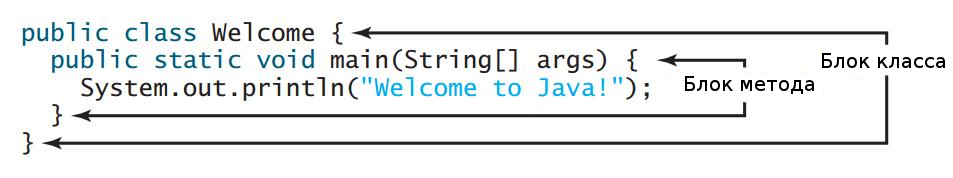
\includegraphics[]{pics/pic2-1.png}
   \caption{Общая форма интерфейса}\label{ris1}
\end{figure}

Если модификатор доступа отсутствует, тогда устанавливается стандартный доступ и интерфейс будет доступным только другим элементам пакета, в котором он объявлен. Когда интерфейс объявлен как public, его может использовать код вне пакета, где он объявлен. В таком случае интерфейс должен быть единственным открытым интерфейсом, объявленным в файле, а файл должен иметь то же имя, что и интерфейс. Имя интерфейса может быть любым допустимым идентификатором. Обратите внимание, что объявленные методы не имеют тела. Они заканчиваются точкой с запятой после списка параметров. По существу это абстрактные методы. Каждый класс, включающий такой интерфейс, обязан реализовывать все методы.

Как показывает общая форма, внутри объявлений интерфейса можно объявлять переменные. Они неявно являются final и static, т.е. не могут изменяться реализующим классом. Они также должны быть инициализированы. Все методы и переменные неявно открыты.

\section{Расширение интерфейсов}
С помощью ключевого слова extends один интерфейс может быть унаследован от другого. Синтаксис используется такой же, как и при наследовании классов. Когда класс реализует интерфейс, унаследованный от другого интерфейса, он должен предоставить реализации для всех методов, требуемых интерфейсами в цепочке наследования. 

\begin{lstlisting}
public interface MyInterface1 {
   // Определение методов
}

public interface MyInterface2 extends MyInterface1 {
   // Определение дополнительных методов
}

public interface MyInterface3 extends MyInterface1, MyInterface2 {
   // Определение дополнительных методов
}
\end{lstlisting}

Здесь интерфейс MyInterface2 расширяет интерфейс MyInterface1 с помощью ключевого слова extends. Таким образом, интерфейс MyInterface2 наследует все методы, определенные в интерфейсе MyInterface1, и может определять дополнительные методы.

Аналогично, интерфейс MyInterface3 расширяет интерфейсы MyInterface1 и MyInterface2, наследуя все их методы и определяя дополнительные методы.

Расширение интерфейсов позволяет создавать более гибкую иерархию интерфейсов, а также улучшать повторное использование кода. Например, можно создать базовый интерфейс с набором общих методов, а затем расширять его для конкретных задач.

Кроме того, интерфейсы в Java могут наследовать методы по умолчанию и статические методы из других интерфейсов. 

\section{Реализация методов по умолчанию в интерфейсах}
В Java 8 была добавлена возможность определения методов по умолчанию в интерфейсах. Методы по умолчанию - это методы, которые имеют реализацию по умолчанию в интерфейсе, но могут быть переопределены в классах, которые реализуют этот интерфейс.

Синтаксис для определения метода по умолчанию выглядит следующим образом:

\begin{lstlisting}
public interface MyInterface {
   // Абстрактный метод
   void abstractMethod();
   
   // Метод по умолчанию
   default void defaultMethod() {
      // Реализация метода по умолчанию
   }
}
\end{lstlisting}

Здесь метод defaultMethod() имеет реализацию по умолчанию с помощью ключевого слова default. Классы, которые реализуют этот интерфейс, могут использовать этот метод по умолчанию или переопределить его, если необходимо. Например:

\begin{lstlisting}
public class MyClass implements MyInterface {
   // Реализация абстрактного метода
   public void abstractMethod() {
      // Реализация метода
   }
   
   // Переопределение метода по умолчанию
   public void defaultMethod() {
      // Реализация переопределенного метода
   }
}
\end{lstlisting}

В этом примере класс MyClass реализует интерфейс MyInterface и предоставляет реализацию для абстрактного метода abstractMethod(). Кроме того, класс переопределяет метод по умолчанию defaultMethod(), предоставляя свою собственную реализацию.

Методы по умолчанию позволяют добавлять новые методы в существующие интерфейсы, не нарушая существующих реализаций, и облегчают разработку библиотек и API.

\newpage
\chapter{Внутренние классы. Типы внутренних классов}

\section{Внутренний класс, его назначение и применимость}
Определение класса может размещаться внутри определения другого класса. Такие классы называются вложенными или внутренними. Область видимости вложенного класса ограничена областью видимости внешнего класса. Поэтому, если вы создадите класс B внутри класса A, то класс B не сможет существовать независимо от класса A. Вложенные классы позволяют группировать классы, логически принадлежащие друг другу, и управлять доступом к ним.

Существуют два типа вложенных класса - статические и нестатические.

Нестатические вложенные классы называют также внутренними классами (inner). Внутренний класс имеет доступ ко всем переменным и методам своего внешнего класса и может непосредственно ссылаться на них.

Внутренние классы создаются внутри окружающего класса:

\begin{lstlisting}
// внешний класс
class Outer {
    int outer_x = 9;
    
    void test() {
        Inner inner = new Inner();
        inner.display();
    }
    
    // внутренний класс
    class Inner {
        void display() {
            Log.i(TAG, outer_x);
        }
    }
}

class MainActivity...{
    // В методе onCreate() активности
    Outer outer = new Outer();
    outer.test();
}
\end{lstlisting}

Внутренний класс Inner определён в области видимости класса Outer. Поэтому любой код в классе Inner может непосредственно обращаться к переменной outer_x. Когда мы создаём экземпляр класса Outer и вызываем метод test(), то создаём также экземпляр класса Inner с вызовом метода display().

Внутренний класс можно определить не только на уровне класса, но и внутри метода или внутри тела цикла.

Если понадобится создать объект внутреннего класса не в статическом методе внешнего класса, тип этого объекта должен задаваться в формате ИмяВнешнегоКласса.ИмяВнутреннегоКласса.

Объект внутреннего класса связан с внешним объектом-создателем и может обращаться к его членам без каких-либо дополнительных описаний. Для внутренних классов доступны все элементы внешнего класса.

Если вам понадобится получить ссылку на объект внешнего класса, запишите имя внешнего класса, за которым следует точка, а затем ключевое слово this.

\section{Основные типы внутренних классов и их характеристики}
Существуют четыре типа внутренних классов в Java:

\begin{enumerate}
\item {\bf Внутренний класс (Inner class)}
Это обычный класс, определенный внутри другого класса. Внутренние классы имеют полный доступ ко всем членам внешнего класса, включая приватные. Они могут быть объявлены с модификаторами доступа, такими как public, private или protected. Внутренние классы могут использоваться для реализации связи "один-к-одному" или создания сложных структур данных.

\item {\bf Статический внутренний класс (Static inner class)}
 Этот класс объявлен как статический внутри другого класса. Он не требует экземпляра внешнего класса для своего создания и может быть использован напрямую. Статические внутренние классы имеют доступ только к статическим членам внешнего класса. Они часто используются для группировки классов, которые логически связаны между собой.

\item {\bf Локальный внутренний класс (Local inner class)}
Это класс, определенный внутри блока кода, такого как метод, конструктор или инициализатор. Локальный внутренний класс имеет доступ ко всем полям и методам внешнего класса, а также к локальным переменным, объявленным в методе, в котором он определен. Локальные внутренние классы могут быть полезными в случаях, когда требуется реализация некоторой функциональности, специфичной для конкретного метода.

\item {\bf Анонимный внутренний класс (Anonymous inner class)}
Это специальный вид локального внутреннего класса, который не имеет имени. Анонимные внутренние классы создаются и объявляются одновременно при создании экземпляра интерфейса или класса-родителя. Они полезны, когда требуется реализовать небольшую функциональность без явного создания отдельного класса. Анонимные внутренние классы могут переопределять методы, определенные в интерфейсе или абстрактном классе, и добавлять свою специфическую реализацию.
\end{enumerate}

Примеры использования внутренних классов могут быть разнообразными. Например, внутренний класс может использоваться для реализации структуры данных, такой как связный список, где каждый узел представлен внутренним классом. Внутренний класс также может быть полезен, когда классу требуется доступ к приватным членам внешнего класса, или для организации кода, связанного с основным классом.


Обратите внимание, что создание экземпляра внутреннего класса требует существования экземпляра внешнего класса.


\section{Отличие вложенных внутренних от вложенных статических классов}

Рассмотрим отличия между вложенными внутренними и вложенными статическими классами в Java.

1. Связь с внешним классом:

\begin{itemize}
  \item Внутренний класс имеет прямой доступ ко всем членам и методам внешнего класса, включая приватные. Он связан с экземпляром внешнего класса и может использовать его поля и методы. Для создания экземпляра внутреннего класса требуется существование экземпляра внешнего класса.
   \item Статический внутренний класс не связан с экземпляром внешнего класса. Он имеет доступ только к статическим членам внешнего класса и не может использовать нестатические поля и методы. Создание экземпляра статического внутреннего класса не требует экземпляра внешнего класса.
\end{itemize}

2. Использование без внешнего класса:

\begin{itemize}
  \item Внутренний класс не может существовать без экземпляра внешнего класса. Это означает, что создание и использование внутреннего класса требует наличия экземпляра внешнего класса.
   \item Статический внутренний класс может существовать независимо от экземпляров внешнего класса. Он может быть использован напрямую без необходимости создания экземпляра внешнего класса.
\end{itemize}

3. Статические члены:

\begin{itemize}
  \item Внутренний класс не может содержать статические поля или методы.
   \item Статический внутренний класс может содержать статические поля и методы, так же как и обычные статические классы.
\end{itemize}

4. Использование в других классах:

\begin{itemize}
  \item Для использования внутреннего класса из других классов необходимо создать экземпляр внешнего класса и использовать его для создания экземпляра внутреннего класса.
   \item Статический внутренний класс может быть использован напрямую без необходимости создания экземпляра внешнего класса.
\end{itemize}

\section{Внутренние классы в локальном методе}
В Java можно объявлять внутренние классы внутри локальных методов. Эти внутренние классы называются локальными внутренними классами или внутренними классами метода (method-local inner classes).

Локальные внутренние классы доступны только внутри метода, в котором они объявлены. Они недоступны за пределами этого метода. 

Данные классы классы могут получать доступ к локальным переменным метода, но только если эти переменные объявлены как final или effectively final. Effective final означает, что значение переменной не изменяется после инициализации. Это требование существует из-за того, что локальные внутренние классы могут использовать эти переменные даже после того, как метод завершил свою работу.

Локальные внутренние классы могут обращаться к методу, в котором они объявлены, включая его параметры и локальные переменные. Это может быть полезно, если внутренний класс должен использовать данные или вызывать методы внешнего метода.

Экземпляры локальных внутренних классов могут быть созданы только внутри метода, в котором они объявлены. Они не могут быть созданы за пределами этого метода.

Локальные внутренние классы могут быть полезны, когда требуется определенная функциональность, связанная с конкретным методом, и не требуется доступ к этой функциональности вне метода. Они помогают упорядочить и структурировать код, улучшают его читаемость и обеспечивают логическую группировку функциональности.

Пример объявления локального внутреннего класса в методе:

\begin{lstlisting}
public class OuterClass {
    public void outerMethod() {
        // Локальный метод
        class LocalInnerClass {
            // Определение локального внутреннего класса
        }
        
        // Использование локального внутреннего класса
        LocalInnerClass inner = new LocalInnerClass();
        // ...
    }
}
\end{lstlisting}

\section{Анонимные классы}
Анонимные классы в Java - это особый вид внутренних классов, которые объявляются без имени. Они используются для создания классов, которые могут быть определены и созданы в одном выражении. Анонимные классы часто используются вместе с интерфейсами или абстрактными классами для реализации или расширения их функциональности.

Ключевые особенностеи анонимных классов:

\begin{enumerate}
\item {\bf Отсутствие имени.}
Анонимные классы не имеют явного имени и объявляются непосредственно в точке использования.

\item {\bf Немедленное создание.}
Анонимные классы создаются в точке объявления и не могут быть повторно использованы в других местах кода.

\item {\bf Расширение или реализация.}
Анонимные классы могут расширять другой класс или реализовывать интерфейс. Они могут переопределять методы из родительского класса или интерфейса.

\item {\bf Ограниченная область видимости.}
Анонимные классы имеют ограниченную область видимости и могут быть использованы только в контексте, где они объявлены.

\item {\bf Использование локальных переменных.}
Анонимные классы могут получать доступ к локальным переменным внешнего метода, но только если эти переменные объявлены как final или effectively final.

Анонимные классы обычно используются для создания одноразовых классов с конкретной функциональностью, которая может быть удобно определена непосредственно на месте использования. Они широко применяются в обработке событий в графическом пользовательском интерфейсе и для реализации слушателей событий.

\end{enumerate}

\begin{lstlisting}
public class AnonymousClassExample {
    public static void main(String[] args) {
        // Создание объекта интерфейса и определение его метода через анонимный класс
        MyInterface myInterface = new MyInterface() {
            @Override
            public void doSomething() {
                System.out.println("Doing something in anonymous class");
            }
        };

        // Вызов метода через объект интерфейса
        myInterface.doSomething();
    }
}

// Интерфейс
interface MyInterface {
    void doSomething();
}
\end{lstlisting}

В этом примере создаем анонимный класс, реализующий интерфейс MyInterface. Анонимный класс определяет метод doSomething(), который выводит сообщение в консоль. Затем создаем объект интерфейса MyInterface с помощью анонимного класса и вызываем его метод doSomething().


\chapter{Перечисляемый тип}

\section{Концепция перечисляемого типа}

Концепция перечисляемого типа (enum) в Java заключается в представлении фиксированного набора именованных констант в виде отдельного типа данных.

Основные аспекты концепции перечисляемого типа в Java включают:

\begin{enumerate}
\item {\bf Определение перечисления.}
С помощью ключевого слова enum определяется новый тип данных, который представляет перечисление. Внутри перечисления определяются константы, разделенные запятыми.

\item {\bf Немедленное создание.}
Анонимные классы создаются в точке объявления и не могут быть повторно использованы в других местах кода.

\item {\bf Именованные константы.}
Константы перечисления представляют возможные значения данного типа. Каждая константа имеет имя и является экземпляром самого перечисления.

\item {\bf Ограниченный набор значений.}
Перечисление представляет ограниченный набор допустимых значений, которые могут принимать переменные этого типа. Значения ограничены набором констант, определенных в перечислении.

\item {\bf Проверка типов.}
Перечисления в Java обеспечивают проверку типов на этапе компиляции. Это означает, что переменные перечисляемого типа могут принимать только значения, определенные в соответствующем перечислении.

\item {\bf Дополнительные функции.}
 Перечисления могут содержать методы, поля и конструкторы, а также переопределять методы, унаследованные от класса Enum. Например, перечисление может иметь методы для получения дополнительной информации о константах.

\end{enumerate}

\section{Перечисляемый тип в Java}

Перечисляемый тип (enum) в Java - это особый тип данных, который представляет фиксированный набор констант. Перечисления позволяют создавать типы данных, которые состоят из ограниченного набора значений, которые не могут быть изменены или расширены во время выполнения программы.

Перечисление объявляется с помощью ключевого слова "enum". Оно может содержать список констант, разделенных запятыми. Каждая константа представляет возможное значение перечисления.

\begin{lstlisting}
enum Season {
    WINTER,
    SPRING,
    SUMMER,
    AUTUMN
}
\end{lstlisting}

 Константы перечисления являются неизменяемыми и статическими. Они могут быть использованы в коде для представления конкретных значений, связанных с перечислением. Перечисления могут содержать методы, поля и конструкторы. Можно определить поведение для каждой константы перечисления. Также существует возможность добавлять стандартные методы, такие как toString(), valueOf(), ordinal() и другие.

 \begin{lstlisting}
enum Season {
    WINTER("Cold"),
    SPRING("Mild"),
    SUMMER("Hot"),
    AUTUMN("Cool");

    private String weather;

    private Season(String weather) {
        this.weather = weather;
    }

    public String getWeather() {
        return weather;
    }
}

\end{lstlisting}

Константы перечислений могут быть использованы в коде, как любые другие константы. Можно сравнивать их с помощью операторов сравнения, использовать в операторах switch, передавать в методы и т.д.

 \begin{lstlisting}
Season currentSeason = Season.SUMMER;

if (currentSeason == Season.SUMMER) {
    System.out.println("It's hot!");
}

switch (currentSeason) {
    case WINTER:
        System.out.println("It's cold.");
        break;
    case SPRING:
        System.out.println("It's mild.");
        break;
    case SUMMER:
        System.out.println("It's hot!");
        break;
    case AUTUMN:
        System.out.println("It's cool.");
        break;
}

\end{lstlisting}

Перечисляемые типы полезны во многих сценариях, когда нужно представить фиксированный набор значений. Они помогают сделать код более читаемым, безопасным и удобным для использования. Например, они могут использоваться для представления дней недели, месяцев, цветов, команд и т.д.

\section{Особенности реализации}

Реализация перечисляемых типов (enum) в Java имеет несколько особенностей.

Перечисление в Java требует публичного конструктора, чтобы создать экземпляры констант. Однако конструкторы перечисления автоматически объявляются как приватные, поэтому доступ к ним ограничен внутри самого перечисления.

Константы перечисления являются статическими объектами, которые создаются автоматически при загрузке класса. Они доступны как статические поля самого перечисления.

Константы перечисления определены в том порядке, в котором они перечислены в коде. При необходимости можно получить порядковый номер каждой константы с помощью метода `ordinal()`, начиная с 0. Каждое перечисление автоматически получает метод `values()`, который возвращает массив, содержащий все константы перечисления в порядке их определения.

Перечисления могут переопределять методы, унаследованные от класса `Enum`. Например, метод `toString()` может быть переопределен для возврата пользовательского представления констант. Перечисление может иметь дополнительные поля и методы, которые могут быть определены для каждой константы. Это позволяет добавлять поведение к конкретным значениям перечисления.

Константы перечисления могут быть сравниваемыми и проверяемыми на равенство с помощью операторов `==` и `equals()`.

\section{Конструкторы и методы перечислений}

Конструкторы перечислений используются для создания экземпляров каждой константы перечисления. Конструкторы перечислений всегда являются приватными и автоматически объявляются компилятором. Они могут принимать аргументы и инициализировать дополнительные поля констант.
 \begin{lstlisting}
enum Day {
    MONDAY("Monday"),
    TUESDAY("Tuesday"),
    WEDNESDAY("Wednesday");

    private String displayName;

    private Day(String displayName) {
        this.displayName = displayName;
    }

    public String getDisplayName() {
        return displayName;
    }
}
\end{lstlisting}

Перечисления могут содержать методы, которые могут быть вызваны для каждой константы перечисления. Эти методы могут выполнять дополнительные операции и возвращать значения.

 \begin{lstlisting}
enum Day {
    MONDAY("Monday"),
    TUESDAY("Tuesday"),
    WEDNESDAY("Wednesday");

    private String displayName;

    private Day(String displayName) {
        this.displayName = displayName;
    }

    public String getDisplayName() {
        return displayName;
    }

    public boolean isWeekend() {
        return this == SATURDAY || this == SUNDAY;
    }
}
\end{lstlisting}

Перечисления могут переопределять методы, унаследованные от класса Enum. Например, метод toString() может быть переопределен для возврата пользовательского представления констант.

 \begin{lstlisting}
enum Day {
    MONDAY("Monday"),
    TUESDAY("Tuesday"),
    WEDNESDAY("Wednesday");

    private String displayName;

    private Day(String displayName) {
        this.displayName = displayName;
    }

    public String getDisplayName() {
        return displayName;
    }

    @Override
    public String toString() {
        return displayName;
    }
}
\end{lstlisting}

Перечисления могут также содержать статические методы, которые могут быть вызваны без создания экземпляра констант. Эти методы могут выполнять общие операции, которые относятся к перечислению в целом.

 \begin{lstlisting}
enum Day {
    MONDAY("Monday"),
    TUESDAY("Tuesday"),
    WEDNESDAY("Wednesday");

    private String displayName;

    private Day(String displayName) {
        this.displayName = displayName;
    }

    public String getDisplayName() {
        return displayName;
    }

    public static Day[] getWeekDays() {
        return new Day[] { MONDAY, TUESDAY, WEDNESDAY };
    }
}
\end{lstlisting}

Конструкторы и методы перечислений позволяют добавлять дополнительную функциональность к перечислениям в Java, делая их более гибкими и мощными для использования в программе.

%--------------------------------------------------------------------------------------------

%\section*{Вопросы и задания для самоконтроля}% Этот раздел будет состоять из вопросов
% и заданий для самоконтроля.
%\addcontentsline{toc}{struct}{Вопросы и задания для самоконтроля}% Эта команда
% добавляет название раздела в раздел <<Содержание>>

%Здесь можете привести список вопросов и заданий для самоконтроля:
%\begin{enumerate}% Эта команда начинает список
%\item Вопрос или задание.
%\item Вопрос или задание.
%\item Вопрос или задание.
%\item Вопрос или задание.
%\end{enumerate}% Эта команда завершает список

%А можете подготовить с помощью программы IrenEditor (см. <<Руководство пользователю>>)
%тестовое задание для самоконтроля, сохранить его в папку
%<<test>>, назвав, например, lk1.exe, и создать на него метку с помощью
%команды (см. <<Руководство пользователю>>): \href{run:test/lk1.exe}{Пройдем тестирование?}

%---------------------------------------------------------------------------------------------
\newpage% Эта команда задает разрыв страницы (начинает новую страницу).
\section*{ПРАКТИЧЕСКОЕ ЗАНЯТИЕ 1}% Эта команда начинает первое практическое занятие.
% Обратите внимание -- практические занятия придется нумеровать вручную.
\addcontentsline{toc}{chapter}{Практическое занятие 1 {\bf Тема занятия}} \vspace{-10pt}% Эти
% команды добавляют тему занятия в раздел <<Содержание>>
\begin{center}% Эта команда выравнивает текст по центру строки.
 {\bf% Эта команда делает шрифт полужирным
 Тема занятия}
\end{center}% Эта команда завершает <<центрирование>> текста.

{\bf Цель:} Сюда можно вписать цель практического занятия.
\\% Эта команда вставляет пустую строку.

Ваш текст.

%--------------------------------------------------------------------------------------------
\newpage% Эта команда начинает новую страницу
\section*{Задания для самостоятельного решения (выполнения)}% Эта команда начинает раздел с
% заданиями для самостоятельной работы
\addcontentsline{toc}{struct}{Задания для самостоятельного решения}% Эта команда добавляет
% название раздела в раздел <<Содержание>>

Ваш текст

\newpage% Эта команда задает новую страницу (разрыв страницы)

%--------------------------------------------------------------------------------------------

\newpage % Эта команда начинает новую страницу



%--------------------------------------------------------------------------------------------

\section*{Вопросы и задания для самоконтроля}% Этот раздел будет состоять из вопросов
% и заданий для самоконтроля.
\addcontentsline{toc}{struct}{Вопросы и задания для самоконтроля}% Эта команда
% добавляет название раздела в раздел <<Содержание>>

Здесь можете привести список вопросов и заданий для самоконтроля:
\begin{enumerate}% Эта команда начинает список
\item Вопрос или задание.
\item Вопрос или задание.
\item Вопрос или задание.
\item Вопрос или задание.
\end{enumerate}% Эта команда завершает список

А можете подготовить с помощью программы IrenEditor (см. <<Руководство пользователю>>)
тестовое задание для самоконтроля, сохранить его в папку
<<test>>, назвав, например, lk1.exe, и создать на него метку с помощью
команды (см. <<Руководство пользователю>>): \href{run:test/lk1.exe}{Пройдем тестирование?}

%---------------------------------------------------------------------------------------------
\newpage% Эта команда задает разрыв страницы (начинает новую страницу).
\section*{ПРАКТИЧЕСКОЕ ЗАНЯТИЕ 2}% Эта команда начинает второе практическое занятие.
% Обратите внимание -- практические занятия придется нумеровать вручную.
\addcontentsline{toc}{chapter}{Практическое занятие 2 {\bf Тема занятия}} \vspace{-10pt}% Эти
% команды добавляют тему занятия в раздел <<Содержание>>
\begin{center}% Эта команда выравнивает текст по центру строки.
 {\bf% Эта команда делает шрифт полужирным
 Тема занятия}
\end{center}% Эта команда завершает <<центрирование>> текста.

{\bf Цель:} Сюда можно вписать цель практического занятия.
\\% Эта команда вставляет пустую строку.

Ваш текст.

%--------------------------------------------------------------------------------------------
\newpage% Эта команда начинает новую страницу
\section*{Задания для самостоятельного решения (выполнения)}% Эта команда начинает раздел с
% заданиями для самостоятельной работы
\addcontentsline{toc}{struct}{Задания для самостоятельного решения}% Эта команда добавляет
% название раздела в раздел <<Содержание>>

Ваш текст

%--------------------------------------------------------------------------------------------

\newpage% Эта команда задает новую страницу (разрыв страницы)


\normalsize\section*{Варианты заданий для индивидуальной работы}% Эта команда создает новый
% раздел, название которого записано в фигурных скобках.
\addcontentsline{toc}{struct}{Варианты заданий для индивидуальной работы} % Эта
% команда добавляет название данного раздела к разделу <<Содержание>>

\begin{center}
   \bf{Вариант 1}
\end{center}

Ваш текст.

\begin{center}
   \bf{Вариант 2}
\end{center}

Ваш текст.

\begin{center}
   \bf{Вариант 3}
\end{center}

Ваш текст.

%--------------------------------------------------------------------------------------------

\newpage% Эта команда задает новую страницу (разрыв страницы)
{\large \section*{Вопросы для подготовки к экзамену и (или) зачету}% Эта команда начинает
% новый раздел, название которого записано в фигурных скобках
\addcontentsline{toc}{struct}{Вопросы для подготовки к экзамену и (или) зачету}% Эта
% команда добавляет название данного раздела к разделу <<Содержание>>

\begin{enumerate}% Эта команда начинает нумерованный список вопросов
 \item Вопрос.
\item Вопрос.
\item Вопрос.
\item Вопрос.
\end{enumerate}% Эта команда завершает нумерованный список вопросов

%--------------------------------------------------------------------------------------------

\newpage% Эта команда задает новую страницу (разрыв страницы)

\addtocontents{toc}{\vspace{15pt}}% Эту команду лучше не менять
\section*{Литература}% Эта команда начинает новый раздел, содержащий список литературы
\addcontentsline{toc}{struct}{Литература}% Эта
% команда добавляет название данного раздела к разделу <<Содержание>>

\itemsep=0pt% Эту команду лучше не менять
\parsep=0pt% Эту команду лучше не менять
\leftmargin=0mm \itemindent=0mm \labelsep=2mm \labelwidth=6mm% Эту команду лучше не менять
\rightmargin=0mm% Эту команду лучше не менять

\begin{enumerate}% Эта команда начинает нумерованный список литературы. На каждый элемент
% списка выставляйте свою метку (с помощью команды \label{name}, где name -- имя метки),
% чтобы иметь возможность ссылаться в тексте на любой элемент списка (см. <<Руководство
% пользователю>>.

\item\label{r8} Львовский,~С.М. Набор и вёрстка в пакете~\LaTeX.~---
М., Космосинформ, 1994.

\item\label{r1} Кнут,~Д. Всё про \TeX.~--- Протвино, RD\TeX, 1993.

\end{enumerate}% Эта команда завершает нумерованный список литературы.

%----------------------------------------------------------------------------------------

\label{pages_total}% Это метка на последнюю страницу электронного учебника. Она нужна для
% корректной работы интерактивного учебника

\end{document}% Эта команда завершает рабочий (исходный) файл электронного учебника
